\documentclass[11pt,twoside,a4paper]{article}
% http://www-h.eng.cam.ac.uk/help/tpl/textprocessing/latex_maths+pix/node6.html symboles de math
% http://fr.wikibooks.org/wiki/Programmation_LaTeX Programmation latex (wikibook)
%=========================== En-Tete =================================
%--- Insertion de paquetages (optionnel) ---
\usepackage[french]{babel}   % pour dire que le texte est en fran{\'e}ais
\usepackage{a4}	             % pour la taille   
\usepackage[T1]{fontenc}     % pour les font postscript
\usepackage{epsfig}          % pour gerer les images
%\usepackage{psfig}
\usepackage{amsmath, amsthm} % tres bon mode mathematique
\usepackage{amsfonts,amssymb}% permet la definition des ensembles
\usepackage{float}           % pour le placement des figure
\usepackage{verbatim}

\usepackage{longtable} % pour les tableaux de plusieurs pages

\usepackage[table]{xcolor} % couleur de fond des cellules de tableaux

\usepackage{lastpage}

\usepackage{multirow}

\usepackage{multicol} % pour {\'e}crire dans certaines zones en colonnes : \begin{multicols}{nb colonnes}...\end{multicols} 

% \usepackage[top=1.5cm, bottom=1.5cm, left=1.5cm, right=1.5cm]{geometry}
% gauche, haut, droite, bas, entete, ente2txt, pied, txt2pied
\usepackage{vmargin}
\setmarginsrb{1.0cm}{1.0cm}{1.0cm}{1.0cm}{15pt}{3pt}{60pt}{27pt}

\usepackage{lscape} % changement orientation page
%\usepackage{frbib} % enlever pour obtenir references en anglais
% --- style de page (pour les en-tete) ---
\pagestyle{headings}

% % % en-tete et pieds de page configurables : fancyhdr.sty

% http://www.trustonme.net/didactels/250.html

% http://ww3.ac-poitiers.fr/math/tex/pratique/entete/entete.htm
% http://www.ctan.org/tex-archive/macros/latex/contrib/fancyhdr/fancyhdr.pdf
\usepackage{fancyhdr}
\pagestyle{fancy}
% \newcommand{\chaptermark}[1]{\markboth{#1}{}}
% \newcommand{\sectionmark}[1]{\markright{\thesection\ #1}}
\fancyhf{}
\fancyhead[LE,RO]{ }
%% \fancyhead[LO]{\bfseries\rightmark}
%% \fancyhead[RE]{\bfseries\leftmark}
\fancyfoot[LE]{\thepage /\pageref{LastPage} \hfill
	Le logiciel d{\'e}vore le monde... depuis les {\'E}tats-Unis
\hfill 
\includegraphics[width=0.5cm]{img/logo_glider.png} }
\fancyfoot[RO]{
\includegraphics[width=0.5cm]{img/logo_glider.png} \hfill
	Le logiciel d{\'e}vore le monde... depuis les {\'E}tats-Unis
\hfill \thepage /\pageref{LastPage}}
\renewcommand{\headrulewidth}{0.5pt}
\renewcommand{\footrulewidth}{0.5pt}
\addtolength{\headheight}{0.5pt}
\fancypagestyle{plain}{
	\fancyhead{}
	\renewcommand{\headrulewidth}{0pt}
}

\renewcommand{\headrulewidth}{0.25pt}
\renewcommand{\footrulewidth}{0.5pt}
%% \setlength{\headheight}{85pt}
% \addtolength{\headheight}{0.5pt}
% \fancypagestyle{plain}{
% 	\fancyhead{}
% 	\fancyfoot{}
% 	\renewcommand{\headrulewidth}{0pt}
% }

%--- Definitions de nouvelles commandes ---
\newcommand{\N}{\mathbb{N}} % les entiers naturels

%% \usepackage{endnotes}

%============================= Corps =================================
\begin{document}

\setlength\parindent{0pt}

\texttt{\small http://colin-verdier.com/le-logiciel-devore-le-monde-depuis-les-etats-unis/}~\\

\textbf{\Large Le logiciel d{\'e}vore le monde... depuis les {\'E}tats-Unis}~\\
\emph{Posted on 4 novembre 2012 by Nicolas Colin}~\\

\begin{minipage}[h]{5.00cm}
	
\includegraphics[width=4.85cm]{img/pacman.png}
\end{minipage} \hfill \begin{minipage}[h]{13cm}
	\texttt{Marc Andreessen}~\footnotemark, concepteur du premier navigateur graphique, \texttt{Mosaic}~\footnotemark, et d{\'e}sormais l'un des plus influents \texttt{\emph{venture capitalists}}~\footnotemark du march{\'e}, a pour habitude de d{\'e}clarer que <<\emph{le logiciel d{\'e}vore le monde}>>. Il a explicit{\'e} sa formule dans un \texttt{article}~\footnotemark paru l'ann{\'e}e derni{\`e}re dans le \emph{Wall Street Journal} : l'{\`e}re du \emph{pure playing} est termin{\'e}e ; d{\'e}sormais le logiciel va s'immiscer dans tous les secteurs de l'{\'e}conomie, s'hybrider avec le mat{\'e}riel et affecter les positions et les niveaux de marge de tous les acteurs en place.
\end{minipage} ~\\~\\
\footnotetext[1]{\texttt{http://en.wikipedia.org/wiki/Marc\_Andreessen}}
\footnotetext[2]{\texttt{http://en.wikipedia.org/wiki/Mosaic\_(web\_browser)}}
\footnotetext[3]{\texttt{http://a16z.com/}}
\footnotetext[4]{\texttt{http://online.wsj.com/article/SB10001424053111903480904576512250915629460.html}}

\begin{minipage}[h]{12cm}
	\texttt{Apple, Google et Amazon}~\footnotemark sont exemplaires des disruptions que le logiciel inflige {\`a} diff{\'e}rents secteurs de l'{\'e}conomie. Avec l'iPod et iTunes, Apple a impos{\'e} un nouveau mod{\`e}le {\'e}conomique {\`a} \texttt{l'industrie de la musique}~\footnotemark. Avec son moteur de recherche et la r{\'e}gie AdWords, Google a capt{\'e} une part croissante des recettes publicitaires en ligne et g{\'e}n{\'e}ralis{\'e} la mesure de la performance dans ce secteur, \texttt{bouleversant au passage les mod{\`e}les {\'e}conomiques}~\footnotemark de tous les acteurs qui d{\'e}pendent de la publicit{\'e}, notamment les m{\'e}dias. Amazon a d{\'e}ploy{\'e} une infrastructure globale et ouverte pour la vente en ligne et, en \texttt{raccourcissant sans cesse ses d{\'e}lais de livraison}~\footnotemark, s'appr{\^e}te {\`a} s'attaquer aux positions des g{\'e}ants de la grande distribution. Wal-Mart l'a bien compris et a d{\'e}cid{\'e} de prendre les devants en \texttt{cessant de vendre les terminaux Kindle}~\footnotemark, sugg{\'e}rant une guerre {\`a} venir entre le g{\'e}ant de la grande distribution et celui de la vente en ligne. Le vainqueur, heureusement ou malheureusement, est connu d'avance -- apr{\`e}s tout, Wal-Mart a, \texttt{{\`a} l'{\'e}poque}~\footnotemark, lui-m{\^e}me provoqu{\'e} la faillite de la plupart de ses concurrents dans la distribution alimentaire aux Etats-Unis.
\end{minipage} \hfill \begin{minipage}[h]{6.00cm}
	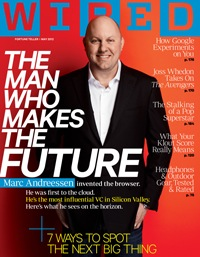
\includegraphics[width=5.85cm]{img/2005-new.jpg}
\end{minipage} ~\\~\\
\footnotetext[5]{\texttt{http://colin-verdier.com/amazon-google-facebook-lart-de-la-guerre-a-lage-de-la-multitude/}}
\footnotetext[6]{\texttt{http://www.amazon.fr/Fortunes-Fool-Bronfman-Warner-Industry/dp/0743269985}}
\footnotetext[7]{\texttt{http://www.amazon.fr/Googled-End-World-We-Know/dp/0753522438/}}
\footnotetext[8]{\texttt{http://www.slate.com/articles/business/small\_business/2012/07/amazon\_same\_day\_delivery\_how\_the\_e\_commerce\_giant\_will\_destroy\_local\_retail\_.html}}
\footnotetext[9]{\texttt{http://www.nytimes.com/2012/09/21/business/wal-mart-stores-dropping-amazon-kindle-tablets-and-e-readers.html}}
\footnotetext[10]{\texttt{http://www.walmarteffectbook.com/}}

\begin{minipage}[h]{8.00cm}
	
\includegraphics[width=7.85cm]{img/amazon-walmart.jpg}
\end{minipage} \hfill \begin{minipage}[h]{10cm}
	Le logiciel a donc d'ores et d{\'e}j{\`a} transform{\'e} quatre grands secteurs de l'{\'e}conomie : les industries culturelles, la publicit{\'e}, les m{\'e}dias et la vente de d{\'e}tail. Mais, comme nous le rappelle Marc Andreessen, il ne va pas s'arr{\^e}ter l{\`a}. Toutes les industries sont concern{\'e}es par la voracit{\'e} du logiciel, y compris celles dont la composante mat{\'e}rielle est irr{\'e}ductible :
\end{minipage} ~\\~\\

%% \clearpage

\setlength\parindent{15pt}
\begin{itemize}
	\item le march{\'e} du \textbf{tourisme} est depuis longtemps transform{\'e} par le logiciel. Nous connaissons les \texttt{TripAdvisor}~\footnote{\texttt{http://www.tripadvisor.com/}}, \texttt{Expedia}~\footnote{\texttt{http://www.expedia.fr/}} et autres \texttt{Booking.com}~\footnote{\texttt{http://www.booking.com/}}, sans lesquels nous ne saurions plus planifier nos voyages ni r{\'e}server de billets d'avions ou de chambres d'h{\^o}tels. Nous connaissons moins les plateformes de gestion de r{\'e}servations telles qu'\texttt{Amadeus}~\footnote{\texttt{http://www.amadeus.com/amadeus/amadeus.html}}, qui forment l'infrastructure logicielle mondiale du march{\'e} du transport a{\'e}rien. Et le tourisme n'a pas fini d'{\^e}tre boulevers{\'e} par le logiciel : par exemple, \texttt{HipMunk}~\footnote{\texttt{http://www.hipmunk.com/}} ou \texttt{Capitaine Train}~\footnote{\texttt{http://www.capitainetrain.com/}} le bouleversent par le design, ou encore la d{\'e}ferlante \texttt{AirBnB}~\footnote{\texttt{http://www.businessweek.com/articles/2012-10-25/airbnb-coursera-and-uber-the-rise-of-the-disruption-economy}} agrandit consid{\'e}rablement le march{\'e} en mettant les h{\^o}tels en concurrence avec les particuliers qui louent leurs chambres inoccup{\'e}es ;
	\item les \textbf{transports} sont l'une des autres transformations en cours. {\`A} l'aide d'une application simple et s{\'e}duisante, la soci{\'e}t{\'e} \texttt{Uber}~\footnote{\texttt{http://en.wikipedia.org/wiki/Uber\_(company)}}, succ{\`e}s quasi-instantan{\'e}, pr{\'e}pare une rude concurrence aux soci{\'e}t{\'e}s de taxi en imposant une disponibilit{\'e} et une qualit{\'e} de service jusqu'ici r{\'e}serv{\'e}e aux clients des chauffeurs de ma{\^i}tre. \texttt{Waze}~\footnote{\texttt{http://www.waze.com/}}, GPS collaboratif, propose d'optimiser les trajets en ville en s'appuyant exclusivement sur les donn{\'e}es d'utilisation de la communaut{\'e}, y compris pour dessiner les fonds de cartes. La \texttt{Google Car}~\footnote{\texttt{http://www.wired.com/magazine/2012/01/ff\_autonomouscars/}} montre la voie aux constructeurs automobiles pour la mise au point des futures voitures sans chauffeur. Et, comme nous le \texttt{sugg{\`e}re}~\footnote{\texttt{http://280.vc/post/17599828612/build-an-autobahn-from-sf-to-la-not-high-speed-rail}} \texttt{Rob Coneybeer}~\footnote{\texttt{http://280.vc/}}, une multitude de voitures sans chauffeur, mises bout {\`a} bout et circulant sur des voies r{\'e}serv{\'e}es, forment une solution de transport collectif bien plus efficiente que le train ;
	\item les \textbf{infrastructures urbaines} font l'objet d'un consid{\'e}rable effort de disruption de la part d'IBM, qui r{\'e}organise progressivement son offre de services autour de la th{\'e}matique des \texttt{\emph{smart cities}}~\footnote{\texttt{http://www.ibm.com/smarterplanet/us/en/smarter\_cities/overview/index.html}} -- jusqu'{\`a} \texttt{supplanter les Veolia ou GDF-Suez}~\footnote{\texttt{http://asmarterplanet.com/blog/2009/02/malta-and-ibm-to-build-worlds-first-national-smart-utility-grid.html}} dans le red{\'e}ploiement du r{\'e}seau de gestion de l'eau sur l'{\^i}le de Malte. Dans son sillage, de nombreuses startups inventent les objets connect{\'e}s qui vont nous aider {\`a} mieux suivre et ma{\^i}triser notre consommation d'{\'e}nergie, notre consommation d'eau, notre gestion des d{\'e}chets, etc. Les \texttt{\emph{smart grids}}~\footnote{\texttt{http://en.wikipedia.org/wiki/Smart\_grid}} propuls{\'e}s par des innovations logicielles vont donc progressivement r{\'e}volutionner la production et la consommation d'{\'e}nergie. Comme nous l'\texttt{explique}~\footnote{\texttt{http://www.tnr.com/blog/plank/109603/power-finally-back-in-manhattan-heres-how-make-sure-it-never-goes-out-again}} \texttt{Tim Wu}~\footnote{\texttt{http://timwu.org/}} dans \texttt{\emph{The New Republic}}~\footnote{\texttt{http://www.tnr.com/}}, ces \emph{smart grids}, form{\'e}s par une multitude d'objets connect{\'e}s, vont devenir l'infrastructure distribu{\'e}e de la production d'{\'e}nergie de demain, une infrastructure plus r{\'e}siliente que nos r{\'e}seaux actuels, qui n'aurait probablement pas fait d{\'e}faut apr{\`e}s le passage de l'ouragan Sandy~\footnote{\texttt{http://www.theatlantic.com/infocus/2012/11/hurricane-sandy-the-aftermath/100397/}} ;
	\item les \textbf{banques} sont saisies depuis longtemps par le logiciel, mais elles se sont prot{\'e}g{\'e}es jusqu'ici de toute disruption par des efforts de \emph{lobbying} fond{\'e}s sur la sensibilit{\'e} des donn{\'e}es qu'elles manipulent et le caract{\`e}re essentiel de leur activit{\'e} pour les {\'e}conomies nationales. Malgr{\'e} tout, le secteur bancaire n'en a plus pour longtemps : le \texttt{pr{\^e}t entre particuliers}~\footnote{\texttt{https://www.lendingclub.com/}} s'attaque aux positions des banques sur le march{\'e} du cr{\'e}dit ; le \texttt{\emph{crowdfunding}}~\footnote{\texttt{http://www.kickstarter.com/}} vient pallier aux d{\'e}ficiences de leurs activit{\'e}s de pr{\^e}t aux entreprises et d'investissement ; les \texttt{solutions de paiement}~\footnote{\texttt{https://www.x.com/}} con\c{c}ues en marge du syst{\`e}me bancaire se multiplient, y compris \emph{via} l'introduction de \texttt{monnaies alternatives}~\footnote{\texttt{http://www.guardian.co.uk/technology/2011/jun/12/bitcoin-online-currency-us-government}} ; m{\^e}me les services de banque de d{\'e}tail vont {\^e}tre transform{\'e}s {\`a} terme gr{\^a}ce aux efforts acharn{\'e}s de soci{\'e}t{\'e}s prometteuses telles que \texttt{Simple}~\footnote{\texttt{http://www.simple.com/}} ;
	~\\ %% ~\\
	\item un consensus se forme d{\'e}j{\`a} sur les prochains secteurs candidats {\`a} la disruption. L'\textbf{{\'e}ducation} est l'un d'entre eux. L'\texttt{endettement des {\'e}tudiants}~\footnote{\texttt{http://www.tnr.com/article/politics/99415/college-tuition-afford-higher-education}} des universit{\'e}s am{\'e}ricaines a atteint un niveau insoutenable, acc{\'e}l{\'e}rant la p{\'e}remption du mod{\`e}le universitaire actuel et intensifiant les efforts d'innovation pour le soumettre {\`a} l'ascendant du logiciel. L'universit{\'e} de \texttt{Stanford}~\footnote{\texttt{http://stanford.edu/}} a r{\'e}cemment pris une \texttt{initiative}~\footnote{\texttt{http://techcrunch.com/2012/05/09/move-over-harvard-and-mit-stanford-has-the-real-revolution-in-education/}} qui pourrait creuser encore plus l'{\'e}cart entre les universit{\'e}s les plus prestigieuses et les autres sur le march{\'e} mondial de l'enseignement sup{\'e}rieur. La soci{\'e}t{\'e} \texttt{Clever}~\footnote{\texttt{http://techcrunch.com/2012/10/22/clever-seed/}} a mis au point une API pour faciliter la connexion au r{\'e}seau des {\'e}coles et l'ouverture des donn{\'e}es du syst{\`e}me {\'e}ducatif ;
	\item la \textbf{sant{\'e}} est l'autre secteur bient{\^o}t expos{\'e} {\`a} une prise en main par l'industrie du logiciel. La \emph{e}-sant{\'e} commence avec le \texttt{\emph{Quantified Self}}~\footnote{\texttt{http://quantifiedself.com/}}, cette pratique consistant {\`a} permettre aux individus de mesurer leurs donn{\'e}es personnelles, notamment de sant{\'e}, et de suivre leur {\'e}volution dans le temps pour en tirer des le\c{c}ons et r{\'e}troagir sur leur comportement. Elle se poursuit par des \texttt{disruptions}~\footnote{\texttt{http://hackingmedicine.mit.edu/}} de l'exercice de la m{\'e}decine ou du remboursement des soins qui sont probablement, bien plus que les m{\'e}dicaments g{\'e}n{\'e}riques ou la chim{\'e}rique \texttt{<<responsabilisation des assur{\'e}s>>}~\footnote{\texttt{http://www.challenges.fr/entreprise/20070208.CHA6458/medecine-sarkozy-veut-responsabiliser-les-patients-avec-une-franchise.html}}, la meilleure promesse de ma{\^i}trise des d{\'e}penses publiques de sant{\'e} sur le long terme. Le logiciel est donc la solution {\`a} \texttt{l'un des plus graves probl{\`e}mes}~\footnote{\texttt{http://fr.wikipedia.org/wiki/Deficit\_de\_la\_Securite\_sociale\_en\_France}} auxquels sont expos{\'e}es nos finances publiques : {\`a} la clef de ces innovations, il y a des milliards d'euros de r{\'e}duction des d{\'e}penses publiques ;
	\item l'\texttt{\textbf{administration}}~\footnote{http://colin-verdier.com/ladministration-comme-plateforme-une-feuille-de-route/} elle-m{\^e}me n'{\'e}chappera pas {\`a} ce rouleur compresseur : anim{\'e}e de la volont{\'e} d'am{\'e}liorer la qualit{\'e} du service rendu aux administr{\'e}s, convaincue du r{\^o}le qu'elle peut jouer dans l'amor\c{c}age d'un {\'e}cosyst{\`e}me d'innovation ou simplement contrainte par l'imp{\'e}ratif de la r{\'e}duction des co{\^u}ts, elle viendra progressivement {\`a} la strat{\'e}gie de \texttt{\emph{government as a platform}}~\footnote{\texttt{http://ofps.oreilly.com/titles/9780596804350/defining\_government\_2\_0\_lessons\_learned\_.html}} -- et laissera des soci{\'e}t{\'e}s logicielles op{\'e}rer {\`a} sa place des services publics sous une forme plus innovante et mieux adapt{\'e}e aux besoins particuliers des administr{\'e}s.
\end{itemize} %% ~\\
\setlength\parindent{0pt}

\begin{minipage}[h]{4.00cm}
	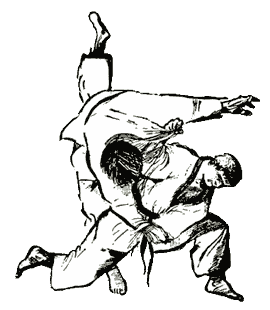
\includegraphics[width=3.85cm]{img/taiotoshi.png}
\end{minipage} \hfill \begin{minipage}[h]{15cm}
	Il est important de prendre la mesure de ces buleversements. Aucun secteur ne sera {\'e}pargn{\'e}. {\`A} toutes les industries, il arrivera ce qui est arriv{\'e} {\`a} la musique, {\`a} la presse, {\`a} la publicit{\'e} et {\`a} la vente de d{\'e}tail. Le fait que les autres secteurs ne puissent {\^e}tre exclusivement immat{\'e}riels ne change rien {\`a} l'affaire. Apple et surtout Amazon ne sont d{\'e}j{\`a} pas des pure players. Ces deux entreprises couronn{\'e}es de succ{\`e}s ont su d{\'e}velopper une offre composite, mi-mat{\'e}rielle, mi-logicielle, qui fait jouer {\`a} plein, sur un march{\'e} essentiellement mat{\'e}riel, le potentiel de disruption du \texttt{logiciel connect{\'e} en r{\'e}seau}~\footnotemark. ~\\
	
	D'o{\`u} vient ce potentiel de disruption ? Lorsqu'un logiciel s'ins{\`e}re dans la cha{\^i}ne de valeur, il capte {\`a} terme l'essentiel de la marge, pour quatre raisons :
\end{minipage}
\footnotetext{\texttt{http://fr.wikipedia.org/wiki/Theoreme\_de\_Bellanger} : \emph{Tout corps plong{\'e} dans un r{\'e}seau devient un r{\'e}seau lui-m{\^e}me}}
\setlength\parindent{15pt}
\begin{itemize}
	\item parce que le logiciel se positionne litt{\'e}ralement \texttt{\emph{over the top}}~\footnote{\texttt{http://www.bbc.co.uk/news/business-17354355}} et devient le maillon qui d{\'e}termine l'allocation des ressources dans la cha{\^i}ne de valeur ;
	\item parce que le logiciel s'ins{\`e}re dans la cha{\^i}ne de valeur prioritairement \texttt{au contact du client ou de l'utilisateur}~\footnote{\texttt{http://www.google.com/about/company/philosophy/}}, ce qui lui conf{\`e}re un avantage suppl{\'e}mentaire dans la captation de la valeur ;
	\item enfin, parce que le logiciel permet de connecter les utilisateurs en r{\'e}seau et d'incorporer au processus de production leurs traces d'utilisation et contributions. C'est le maillon logiciel qui permet {\`a} une cha{\^i}ne de valeur de \texttt{\emph{faire levier de la multitude}}~\footnote{\texttt{http://colin-verdier.com/l-age-de-la-multitude-le-livre/}} et de parvenir aux rendements d'{\'e}chelle consid{\'e}rables qui font la \texttt{scalabilit{\'e}}~\footnote{\texttt{http://en.wikipedia.org/wiki/Scalability}} des mod{\`e}les {\'e}conomiques d'aujourd'hui. Nous en voyons d{\'e}j{\`a} de nombreux exemples : le moteur de recommandation d'Amazon, fond{\'e} sur nos historiques d'achat ; la r{\'e}gie publicitaire AdWords, fond{\'e}e sur nos clics ; l'application Facebook tout enti{\`e}re, fond{\'e}e sur le partage de notre intimit{\'e}. Parce qu'il permet d'incorporer des milliards d'utilisateurs {\`a} la cha{\^i}ne de production, le logiciel atteint des rendements d'{\'e}chelle sans pr{\'e}c{\'e}dent dans l'histoire. Il est donc compr{\'e}hensible qu'il capte l'essentiel de la marge ;
	\item combin{\'e}es, ces trois caract{\'e}ristiques sugg{\`e}rent pourquoi les march{\'e}s logiciels sont toujours concentr{\'e}s. Nous l'avons appris avec Microsoft d{\`e}s les ann{\'e}es 1980. Nous en avons la confirmation avec Google depuis le milieu des ann{\'e}es 2000. Amazon est en train de balayer toute concurrence sur le march{\'e} de la vente en ligne, comme le confirme le \texttt{repli en bon ordre de la FNAC}~\footnote{\texttt{http://www.terrafemina.com/culture/culture-web/articles/19064-fnac--la-musique-ce-sera-sur-itunes.html}}. Il en va de m{\^e}me sur le march{\'e} de l'Internet mobile, que Google et Apple sont vou{\'e}es {\`a} se partager en duopole. Les acteurs du logiciel dominent leurs march{\'e}s et leur position dominante leur permet de capter l'essentiel de la marge.
\end{itemize} ~\\
\setlength\parindent{0pt}

\begin{minipage}[h]{12cm}
	Il n'y a pas d'opposition entre la th{\`e}se d'Andreessen et celle des tenants de la \texttt{renaissance du \emph{hardware}}~\footnotemark, tels \texttt{Rob Coneybeer}~\footnotemark ou \texttt{Paul Graham}~\footnotemark, lequel confirme que les nouvelles promotions de \texttt{Y Combinator}~\footnotemark comptent de plus en plus d'innovateurs dans le \emph{hardware}. Il n'y a pas d'opposition car le \emph{hardware} nouveau est du \texttt{\emph{hardware} connect{\'e}}~\footnotemark : un nouveau point de contact entre le r{\'e}seau et ses utilisateurs, mesur{\'e} et command{\'e} par du logiciel. En revanche, il y a {\`a} cela une cons{\'e}quence majeure : de plus en plus, le fabricant du \emph{hardware} va {\^e}tre un sous-traitant d'un op{\'e}rateur logiciel. Sa marge sera celle d'un sous-traitant, contraint de sans cesse baisser ses prix et de r{\'e}aliser des gains de productivit{\'e}. Le logiciel est aux acteurs de l'{\'e}conomie traditionnelle ce que Wal-Mart est {\`a} ses fournisseurs : un \texttt{rouleau compresseur}~\footnotemark qui r{\'e}duit {\`a} n{\'e}ant la marge d'exploitation et force la \texttt{d{\'e}localisation}~\footnotemark des cha{\^i}nes de production dans des pays o{\`u} le prix de la main-d'oeuvre est plus faible. Dans le partage de la valeur entre les activit{\'e}s traditionnelles et les nouveaux maillons logiciels, ce sont les seconds qui se tailleront la part du lion. --- Il y a deux s{\'e}ries de cons{\'e}quences {\`a} cela. 
\end{minipage} \hfill \begin{minipage}[h]{7.00cm}
	
\includegraphics[width=6.85cm]{img/Nest-Thermostat-2-537x392-300x218.jpg}
\end{minipage}
\footnotetext[51]{\texttt{http://mantellavp.com/a-hardware-renaissance-while-software-eats-the-world/}}
\footnotetext[52]{\texttt{http://280.vc/}}
\footnotetext[53]{\texttt{http://www.paulgraham.com/hw.html}}
\footnotetext[54]{\texttt{http://ycombinator.com/}}
\footnotetext[55]{\texttt{http://en.wikipedia.org/wiki/Internet\_of\_Things}}
\footnotetext[56]{\texttt{http://www.tradereform.org/2012/07/not-made-in-america-top-10-ways-walmart-destroys-us-manufacturing-jobs/}}
\footnotetext[57]{\texttt{http://colin-verdier.com/redresser-lindustrie-automobile-a-lage-de-la-multitude/}}

La premi{\`e}re est d'ordre industriel. Comme d{\'e}j{\`a} {\'e}voqu{\'e}, sur ces march{\'e}s concentr{\'e}s il n'y a pas beaucoup de places {\`a} prendre. Un march{\'e} logiciel est un monopole ou un duopole qui ne m{\'e}nage qu'{\`a} sa marge un peu de place pour des acteurs de niche. Il s'agit par ailleurs de march{\'e}s globaux, car c'est {\`a} l'{\'e}chelle globale qu'on peut parvenir aux rendements d'{\'e}chelle qui font l'essentiel de la valeur... et le pouvoir de march{\'e}. La question est donc celle de la place des entreprises fran\c{c}aises sur ce march{\'e} : certaines s'imposeront-elles comme les g{\'e}ants mondiaux du logiciel dans tel ou tel secteur, ou bien laisseront-elles les entreprises am{\'e}ricaines occuper ces positions strat{\'e}giques en se repliant sur la fabrication de mat{\'e}riel {\`a} bas co{\^u}ts et {\`a} faibles marges (\emph{id est} la \texttt{perspective que nous offre le rapport Gallois}~\footnotemark) ? ~\\
~\footnotetext{\texttt{http://lexpansion.lexpress.fr/economie/competitivite-pourquoi-le-rapport-gallois-ne-restera-pas-lettre-morte\_352950.html}}

L'{\'e}tat des choses est peu rassurant. Confront{\'e}es aux menaces de disruption issues du secteur du logiciel, la plupart des entreprises fran\c{c}aises comprennent qu'il se passe quelque chose mais pr{\'e}f{\`e}rent, pour affronter le danger, nouer des partenariats... avec des soci{\'e}t{\'e}s am{\'e}ricaines ! \texttt{Voyages-SNCF}~\footnotemark n'est pas une position prise par la SNCF sur le march{\'e} du logiciel dans le secteur du tourisme, mais une \texttt{\emph{joint-venture}}~\footnotemark avec la soci{\'e}t{\'e} am{\'e}ricaine Expedia. De m{\^e}me, \texttt{Veolia}~\footnotemark n'a pas investi dans une nouvelle activit{\'e} de gestion d'infrastructure logicielle, mais a pr{\'e}f{\'e}r{\'e} pour cela conclure un \texttt{partenariat avec IBM}~\footnotemark. La FNAC est en partenariat avec \texttt{Kobo}~\footnotemark, soci{\'e}t{\'e} canadienne, pour la vente de liseuses et donc de livres {\'e}lectroniques. On sait comment tout cela finit : {\`a} terme, l'essentiel de la marge sera dans la partie logicielle, donc dans les comptes de soci{\'e}t{\'e}s am{\'e}ricaines (ou canadiennes) et sur les feuilles de paie de salari{\'e}s am{\'e}ricains, tandis que nos ex-champions nationaux se seront transform{\'e}s en vulgaires sous-traitants {\`a} faibles marges d'exploitation. ~\\
\footnotetext[59]{\texttt{http://www.voyages-sncf.com/}}
\footnotetext[60]{\texttt{http://en.wikipedia.org/wiki/Voyages-sncf.com}}
\footnotetext[61]{\texttt{http://www.veolia.fr/}}
\footnotetext[62]{\texttt{http://www.veoliatransdev.com/en/media/press-releases/smarter-mobility.htm}}
\footnotetext[63]{\texttt{http://www.kobobooks.fr/}}

\begin{minipage}[h]{12.00cm}
	Au-del{\`a} de ces accords par lesquels nos soci{\'e}t{\'e}s abandonnent la valeur future {\`a} leurs partenaires {\'e}trangers, un autre danger est d'{\^e}tre tout simplement {\`a} c{\^o}t{\'e} de la plaque. Il n'est pas certain, c'est le moins que l'on puisse dire, que nos g{\'e}ants industriels aient r{\'e}alis{\'e} qu'ils avaient affaire {\`a} \texttt{une concurrence bien plus intense, f{\'e}roce et impr{\'e}visible}~\footnotemark que tout ce qu'ils ont connu par le pass{\'e}. Les g{\'e}ants du logiciel, ceux-l{\`a} m{\^e}me qui d{\'e}vorent les secteurs de l'{\'e}conomie les uns apr{\`e}s les autres, jouent plusieurs coups {\`a} l'avance, mobilisent des quantit{\'e}s consid{\'e}rables de capital, \texttt{ne versent pas de dividendes}~\footnotemark car ils r{\'e}investissent tout (\texttt{ou presque}~\footnotemark) en R\&D, et surtout font levier de la multitude pour atteindre des rendements d'{\'e}chelle sans pr{\'e}c{\'e}dent dans l'histoire de l'industrie.
\end{minipage} \hfill \begin{minipage}[h]{6.00cm}
	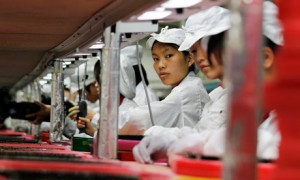
\includegraphics[width=5.85cm]{img/Foxconn-factory-workers-i-008-300x180.jpg}
\end{minipage} ~\\~\\
\footnotetext[64]{\texttt{http://colin-verdier.com/amazon-google-facebook-lart-de-la-guerre-a-lage-de-la-multitude/}}
\footnotetext[65]{\texttt{http://www.quora.com/Why-do-only-a-few-technology-stocks-pay-dividends}}
\footnotetext[66]{\texttt{http://www.guardian.co.uk/news/datablog/2012/mar/19/100-billion-apple}}

\begin{minipage}[h]{6.00cm}
	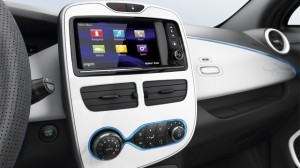
\includegraphics[width=5.85cm]{img/tablette-r-link-renault-zoe-300x168.jpg}
\end{minipage} \hfill \begin{minipage}[h]{12.00cm}
	Face {\`a} cela, Renault travaille {\`a} mettre au point une plateforme logicielle, \texttt{R-link}~\footnotemark, qui est une option payante propos{\'e}e sur certains nouveaux mod{\`e}les seulement. {\`A} ce rythme-l{\`a}, bon courage pour concurrencer Google et Apple sur le march{\'e} des voitures connect{\'e}es ! Pour se pr{\'e}parer {\`a} la disruption logicielle, Renault devrait frapper beaucoup plus vite et plus fort, {\'e}quiper gratuitement tous les mod{\`e}les dans toutes les gammes, et m{\^e}me rappeler les mod{\`e}les anciens pour les connecter en m{\^e}me temps qu'on fait la vidange. De m{\^e}me, alors qu'AT\&T vient d'enrichir son offre d'une \texttt{API d{\'e}ploy{\'e}e en 90 jours}~\footnotemark pour rendre son r{\'e}seau t{\'e}l{\'e}phonique programmable (en r{\'e}action {\`a} l'effort d'innovation de la startup \texttt{Twilio}~\footnotemark, du portefeuille de \texttt{500startups}~\footnotemark), on attend en vain les innovations sur le march{\'e} fran\c{c}ais des t{\'e}l{\'e}communications en dehors de la diversification des forfaits t{\'e}l{\'e}phoniques ou de la baisse des prix forc{\'e}e par \texttt{l'entr{\'e}e de Free sur le march{\'e}}~\footnotemark.
\end{minipage} ~\\~\\
\footnotetext[67]{\texttt{http://www.renault.com/en/innovation/plaisir-et-confort/pages/r-link.aspx}}
\footnotetext[68]{\texttt{http://techcrunch.com/2012/10/18/move-over-twilio-att-integrates-speech-messaging-and-payment-apis-into-appcelerators-developer-platform/}}
\footnotetext[69]{\texttt{http://www.twilio.com/}}
\footnotetext[70]{\texttt{http://500.co/}}
\footnotetext[71]{\texttt{http://www.lefigaro.fr/societes/2012/01/10/04015-20120110ARTFIG00359-free-mobile-casse-les-prix-avec-deux-forfaits.php}}

\begin{minipage}[h]{12.00cm}
	Bien s{\^u}r, il n'y a l{\`a} rien de nouveau depuis l'\texttt{ouvrage fondateur}~\footnotemark de \texttt{Clayton Christensen}~\footnotemark : les grands groupes {\'e}prouvent les plus grandes difficult{\'e}s {\`a} anticiper et {\`a} s'emparer des innovations de rupture. Mais la France, avec sa tradition colbertiste et la discipline d'ex{\'e}cution de ses champions nationaux, si proches du pouvoir politique, n'est-elle pas la seule (avec la \texttt{Cor{\'e}e du Sud}~\footnotemark peut-{\^e}tre) {\`a} pouvoir forcer ses grands groupes {\`a} se faire violence et {\`a} relever les d{\'e}fis d'apr{\`e}s la r{\'e}volution num{\'e}rique ? Il faut en effet consid{\'e}rer la \texttt{th{\`e}se de Scott D. Anthony}~\footnotemark : puisqu'une poign{\'e}e de soci{\'e}t{\'e}s logicielles, devenues des g{\'e}ants, ont pris une avance impossible {\`a} rattraper, l'innovation de rupture doit maintenant retrouver sa place dans les strat{\'e}gies des grands groupes, seuls {\`a} pouvoir mobiliser suffisamment de ressources dans de courts d{\'e}lais pour forcer des disruptions sur leurs march{\'e}s... plut{\^o}t que d'{\^e}tre d{\'e}vor{\'e}s par un logiciel d{\'e}velopp{\'e} par d'autres !
\end{minipage} \hfill \begin{minipage}[h]{6.00cm}
	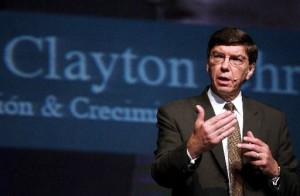
\includegraphics[width=5.85cm]{img/clayton-christensen-02-300x196.jpg}
\end{minipage} ~\\~\\
\footnotetext[72]{\texttt{http://www.amazon.com/Innovators-Dilemma-Revolutionary-Change-Business/dp/0062060244}}
\footnotetext[73]{\texttt{http://www.claytonchristensen.com/}}
\footnotetext[74]{\texttt{http://images.businessweek.com/ss/09/03/0312\_innovative\_countries/30.htm}}
\footnotetext[75]{\texttt{http://hbr.org/2012/09/the-new-corporate-garage/ar/1}}

Nos soci{\'e}t{\'e}s logicielles (\texttt{Dassault Syst{\`e}mes}~\footnote{\texttt{http://www.3ds.com/fr/}}, \texttt{Atos}~\footnote{\texttt{http://fr.atos.net/fr-fr/}}, \texttt{CapGemini}~\footnote{\texttt{http://www.fr.capgemini.com/}}...) affirmeront avec force que, bien s{\^u}r, elles s'efforcent de mieux se positionner dans la cha{\^i}ne de valeur. Mais les probl{\`e}mes sont syst{\'e}miques. Il y a maintes raisons {\`a} cette incapacit{\'e} de soci{\'e}t{\'e}s fran\c{c}aises {\`a} s'imposer sur des march{\'e}s logiciels globaux. ~\\

Par exemple, pour innover en rupture dans les grands groupes comme pour les startups, il faut des investissements consid{\'e}rables, r{\'e}alis{\'e}s dans des d{\'e}lais tr{\`e}s courts. C'est ce genre d'efforts que font les g{\'e}ants du logiciel aux Etats-Unis pour acqu{\'e}rir et consolider leurs positions : \texttt{Facebook a investi depuis sa cr{\'e}ation pr{\`e}s de \emph{1,5 milliard de dollars}}~\footnote{\texttt{http://www.crunchbase.com/company/facebook}}, sans avoir prouv{\'e} sa capacit{\'e} {\`a} g{\'e}n{\'e}rer des revenus \texttt{{\`a} hauteur de son cours d'introduction en bourse}~\footnote{\texttt{http://www.mondaynote.com/2012/02/05/strange-facebook-economics/}}. \texttt{Palantir}~\footnote{\texttt{http://www.crunchbase.com/company/palantir-technologies}}, soci{\'e}t{\'e} fond{\'e}e par \texttt{Peter Thiel}~\footnote{\texttt{http://www.newyorker.com/reporting/2011/11/28/111128fa\_fact\_packer}}, a lev{\'e}, depuis sa cr{\'e}ation en 2004, \emph{301 millions de dollars} sans encore avoir stabilis{\'e} son mod{\`e}le {\'e}conomique. C'est la finalit{\'e} du venture capital que de mobiliser de telles sommes en dehors des grandes organisations pour aider des entreprises innovantes {\`a} prendre des positions strat{\'e}giques sur d'immenses march{\'e}s qu'elles contribuent {\`a} transformer voire {\`a} cr{\'e}er, avant m{\^e}me de prouver leur profitabilit{\'e}. Comme nous le rappelle Scott D. Anthony dans \texttt{l'article r{\'e}f{\'e}renc{\'e} plus haut}~\footnote{\texttt{http://hbr.org/2012/09/the-new-corporate-garage/ar/1}}, ~\\

\begin{minipage}[h]{14.00cm}
    \emph{The restless individualism of baby boomers clashed with increasingly hierarchical organizations. Innovators began to leave companies, band with like-minded ``rebels'', and form new companies. \textbf{Given the scale required to innovate, however, these rebels needed new forms of funding. Hence the emergence of the VC-backed start-up. } }
\end{minipage} \hfill \begin{minipage}[h]{2cm}
	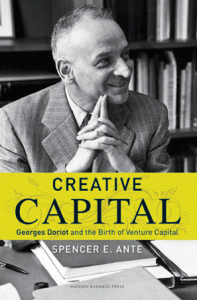
\includegraphics[width=1.85cm]{img/creative-capital-cr-197x300.png}
\end{minipage} ~\\

Pour faire {\'e}merger des champions logiciels, il ne faut pas seulement du \emph{venture capital}, il faut aussi un environnement juridique favorable {\`a} l'{\'e}mergence d'applications innovantes, qui sont les plateformes logicielles mondiales de demain. M{\^e}me si la disruption vient d'un grand groupe, ce dernier est souvent aiguillonn{\'e} par une startup (laquelle est alors rachet{\'e}e par le \emph{second mover}), comme le montre l'\texttt{exemple d'AT\&T et de Twilio}~\footnote{\texttt{http://techcrunch.com/2012/10/18/move-over-twilio-att-integrates-speech-messaging-and-payment-apis-into-appcelerators-developer-platform/}}. Or de nombreux indices nous sugg{\`e}rent que la France entrave l'essor de l'innovation logicielle : \texttt{confusion entre recherche et d{\'e}veloppement et innovation}~\footnote{\texttt{http://www.industrie.com/it/quelles-sont-les-entreprises-les-plus-innovantes.13978}} ; \texttt{obsession du brevet et de la propri{\'e}t{\'e} intellectuelle}~\footnote{\texttt{http://techcrunch.com/2010/08/07/why-we-need-to-abolish-software-patents/}} ; frilosit{\'e} des grands groupes (voyez le \texttt{parcours du combattant de Capitaine Train}~\footnote{\texttt{http://www.capitainetrain.com/about}} pour mettre en place son application de r{\'e}servation de billets de train) ; captation des comp{\'e}tences informatiques, par ailleurs \texttt{d{\'e}valoris{\'e}es}~\footnote{\texttt{http://peerdal.blogspot.fr/2011/01/computer-science-and-engineers-bad.html}}, par les SSII ; fonctionnement du march{\'e} du travail et des assurances sociales inadapt{\'e} aux cycles courts d'innovation ; multiplication des obstacles juridiques au r{\'e}f{\'e}rencement des contenus ou {\`a} l'exploitation des donn{\'e}es (dans l'\texttt{{\'e}ducation}~\footnote{\texttt{http://secouezlecours.wordpress.com/2012/10/21/un-pas-en-avant-trois-pas-en-arriere-la-twittclasse-de-la-roche-sur-foron-ne-repond-plus/}}, dans la \texttt{sant{\'e}}~\footnote{\texttt{http://www.journaldunet.com/web-tech/start-up/fourmi-sante-honoraires-0912.shtml}} et peut-{\^e}tre bient{\^o}t dans les \texttt{m{\'e}dias)}~\footnote{\texttt{http://www.lesechos.fr/entreprises-secteurs/tech-medias/actu/0202246753016-les-editeurs-veulent-leur-lex-google-358789.php}} ; fiscalit{\'e} \texttt{d{\'e}favorable au \emph{venture capital}}~\footnote{\texttt{http://www.latribune.fr/technos-medias/internet/20121013trib000724671/dans-le-capital-risque-on-perd-plus-souvent-que-l-on-ne-gagne.html}} ; multiples r{\'e}glementations sectorielles constituant des \texttt{barri{\`e}res {\`a} l'entr{\'e}e infranchissables pour les nouveaux acteurs}~\footnote{\texttt{http://colin-verdier.com/le-droit-et-les-proprietes-emergentes/}}, par ailleurs sous-financ{\'e}s. ~\\

\clearpage

Tout cela mis ensemble forme un {\'e}cosyst{\`e}me hostile {\`a} l'innovation : les innovateurs fran\c{c}ais doivent surmonter plus d'obstacles que leurs concurrents {\'e}trangers, et les venture capitalists pr{\'e}f{\`e}rent parier sur ces derniers plut{\^o}t que sur nos startups fran\c{c}aises. Qui, dans ces conditions, prendra les positions dominantes sur les march{\'e}s logiciels globaux de demain ? Les Microsoft, Apple, Google et Amazon de la sant{\'e}, de l'{\'e}ducation, de l'automobile seront-ils fran\c{c}ais ou am{\'e}ricains ? ~\\

\begin{minipage}[h]{5.00cm}
	
\includegraphics[width=4.85cm]{img/1137572-213x300.jpg}
\end{minipage} \hfill \begin{minipage}[h]{14.00cm}
	La deuxi{\`e}me s{\'e}rie de cons{\'e}quences est d'ordre fiscal. Ce n'est \texttt{pas ici}~\footnotemark le lieu pour s'{\'e}tendre sur ce sujet, mais il est facile de comprendre que si la partie logicielle des activit{\'e}s dans tous les secteurs est op{\'e}r{\'e} par des soci{\'e}t{\'e}s {\'e}trang{\`e}res, alors l'imp{\^o}t sur les soci{\'e}t{\'e}s et la TVA (jusqu'en 2019 sur les prestations de service immat{\'e}riel) sur ces activit{\'e}s, qui captent l'essentiel de la marge, seront \texttt{pay{\'e}s {\`a} l'{\'e}tranger plut{\^o}t qu'en France}~\footnotemark. Comme le \texttt{secteur financier}~\footnotemark, le secteur logiciel, parce que ses actifs et ses prestations sont immat{\'e}riels, se pr{\^e}te tout particuli{\`e}rement {\`a} l'\texttt{optimisation fiscale}~\footnotemark. Dans la bataille pour la \texttt{localisation des bases fiscales}~\footnotemark, mieux vaut favoriser l'{\'e}mergence en France d'acteurs dominants sur les march{\'e}s logiciels globaux plut{\^o}t que de laisser les marges de toutes les cha{\^i}nes de valeur dans tous les secteurs, y compris ceux dans lesquels nous sommes aujourd'hui les plus forts (voyez Veolia, Renault ou nos \texttt{g{\'e}ants de la grande distribution}~\footnotemark), s'{\'e}chapper dans les comptes de soci{\'e}t{\'e}s {\'e}trang{\`e}res {\`a} la suite de disruptions logicielles et d'une restructuration en profondeur de la cha{\^i}ne de valeur. C'est ce message que j'ai cherch{\'e} {\`a} faire passer dans mon intervention mardi dernier aux \texttt{Rencontres parlementaires sur l'{\'e}conomie num{\'e}rique}~\footnotemark. \texttt{{\`A} suivre}~\footnotemark !
\end{minipage} ~\\
\footnotetext[94]{\texttt{http://www.economie.gouv.fr/economie/fiscalite-leconomie-numerique-creation-dune-mission-dexpertise}}
\footnotetext[95]{\texttt{http://www.senat.fr/leg/ppl11-682.html}}
\footnotetext[96]{\texttt{http://ec.europa.eu/taxation\_customs/taxation/other\_taxes/financial\_sector/index\_en.htm}}
\footnotetext[97]{\texttt{http://www.bloomberg.com/news/2010-10-21/google-2-4-rate-shows-how-60-billion-u-s-revenue-lost-to-tax-loopholes.html}}
\footnotetext[98]{\texttt{http://www.oecd.org/ctp/baseerosionandprofitshifting.htm}}
\footnotetext[99]{\texttt{http://fr.wikipedia.org/wiki/Groupe\_Auchan}}
\footnotetext[100]{\texttt{http://www.gazettedupalais.com/services/actualites/agenda/e-docs/rencontres\_parlementaires\_sur\_leconomie\_numerique\_pour\_une\_relance\_durable\_de\_leconomie\_numerique\_/document\_agenda.phtml?cle\_doc=000021D4}}
\footnotetext[101]{\texttt{http://www.lemonde.fr/politique/article/2012/09/18/votee-retardee-supprimee-petite-histoire-de-la-taxe-google\_1761318\_823448.html}}

Vous {\^e}tes la multitude !

\end{document}
